% Options for packages loaded elsewhere
\PassOptionsToPackage{unicode}{hyperref}
\PassOptionsToPackage{hyphens}{url}
\PassOptionsToPackage{dvipsnames,svgnames,x11names}{xcolor}
%
\documentclass[
  letterpaper,
  DIV=11,
  numbers=noendperiod]{scrartcl}

\usepackage{amsmath,amssymb}
\usepackage{lmodern}
\usepackage{iftex}
\ifPDFTeX
  \usepackage[T1]{fontenc}
  \usepackage[utf8]{inputenc}
  \usepackage{textcomp} % provide euro and other symbols
\else % if luatex or xetex
  \usepackage{unicode-math}
  \defaultfontfeatures{Scale=MatchLowercase}
  \defaultfontfeatures[\rmfamily]{Ligatures=TeX,Scale=1}
\fi
% Use upquote if available, for straight quotes in verbatim environments
\IfFileExists{upquote.sty}{\usepackage{upquote}}{}
\IfFileExists{microtype.sty}{% use microtype if available
  \usepackage[]{microtype}
  \UseMicrotypeSet[protrusion]{basicmath} % disable protrusion for tt fonts
}{}
\makeatletter
\@ifundefined{KOMAClassName}{% if non-KOMA class
  \IfFileExists{parskip.sty}{%
    \usepackage{parskip}
  }{% else
    \setlength{\parindent}{0pt}
    \setlength{\parskip}{6pt plus 2pt minus 1pt}}
}{% if KOMA class
  \KOMAoptions{parskip=half}}
\makeatother
\usepackage{xcolor}
\setlength{\emergencystretch}{3em} % prevent overfull lines
\setcounter{secnumdepth}{5}
% Make \paragraph and \subparagraph free-standing
\ifx\paragraph\undefined\else
  \let\oldparagraph\paragraph
  \renewcommand{\paragraph}[1]{\oldparagraph{#1}\mbox{}}
\fi
\ifx\subparagraph\undefined\else
  \let\oldsubparagraph\subparagraph
  \renewcommand{\subparagraph}[1]{\oldsubparagraph{#1}\mbox{}}
\fi

\usepackage{color}
\usepackage{fancyvrb}
\newcommand{\VerbBar}{|}
\newcommand{\VERB}{\Verb[commandchars=\\\{\}]}
\DefineVerbatimEnvironment{Highlighting}{Verbatim}{commandchars=\\\{\}}
% Add ',fontsize=\small' for more characters per line
\usepackage{framed}
\definecolor{shadecolor}{RGB}{241,243,245}
\newenvironment{Shaded}{\begin{snugshade}}{\end{snugshade}}
\newcommand{\AlertTok}[1]{\textcolor[rgb]{0.68,0.00,0.00}{#1}}
\newcommand{\AnnotationTok}[1]{\textcolor[rgb]{0.37,0.37,0.37}{#1}}
\newcommand{\AttributeTok}[1]{\textcolor[rgb]{0.40,0.45,0.13}{#1}}
\newcommand{\BaseNTok}[1]{\textcolor[rgb]{0.68,0.00,0.00}{#1}}
\newcommand{\BuiltInTok}[1]{\textcolor[rgb]{0.00,0.23,0.31}{#1}}
\newcommand{\CharTok}[1]{\textcolor[rgb]{0.13,0.47,0.30}{#1}}
\newcommand{\CommentTok}[1]{\textcolor[rgb]{0.37,0.37,0.37}{#1}}
\newcommand{\CommentVarTok}[1]{\textcolor[rgb]{0.37,0.37,0.37}{\textit{#1}}}
\newcommand{\ConstantTok}[1]{\textcolor[rgb]{0.56,0.35,0.01}{#1}}
\newcommand{\ControlFlowTok}[1]{\textcolor[rgb]{0.00,0.23,0.31}{#1}}
\newcommand{\DataTypeTok}[1]{\textcolor[rgb]{0.68,0.00,0.00}{#1}}
\newcommand{\DecValTok}[1]{\textcolor[rgb]{0.68,0.00,0.00}{#1}}
\newcommand{\DocumentationTok}[1]{\textcolor[rgb]{0.37,0.37,0.37}{\textit{#1}}}
\newcommand{\ErrorTok}[1]{\textcolor[rgb]{0.68,0.00,0.00}{#1}}
\newcommand{\ExtensionTok}[1]{\textcolor[rgb]{0.00,0.23,0.31}{#1}}
\newcommand{\FloatTok}[1]{\textcolor[rgb]{0.68,0.00,0.00}{#1}}
\newcommand{\FunctionTok}[1]{\textcolor[rgb]{0.28,0.35,0.67}{#1}}
\newcommand{\ImportTok}[1]{\textcolor[rgb]{0.00,0.46,0.62}{#1}}
\newcommand{\InformationTok}[1]{\textcolor[rgb]{0.37,0.37,0.37}{#1}}
\newcommand{\KeywordTok}[1]{\textcolor[rgb]{0.00,0.23,0.31}{#1}}
\newcommand{\NormalTok}[1]{\textcolor[rgb]{0.00,0.23,0.31}{#1}}
\newcommand{\OperatorTok}[1]{\textcolor[rgb]{0.37,0.37,0.37}{#1}}
\newcommand{\OtherTok}[1]{\textcolor[rgb]{0.00,0.23,0.31}{#1}}
\newcommand{\PreprocessorTok}[1]{\textcolor[rgb]{0.68,0.00,0.00}{#1}}
\newcommand{\RegionMarkerTok}[1]{\textcolor[rgb]{0.00,0.23,0.31}{#1}}
\newcommand{\SpecialCharTok}[1]{\textcolor[rgb]{0.37,0.37,0.37}{#1}}
\newcommand{\SpecialStringTok}[1]{\textcolor[rgb]{0.13,0.47,0.30}{#1}}
\newcommand{\StringTok}[1]{\textcolor[rgb]{0.13,0.47,0.30}{#1}}
\newcommand{\VariableTok}[1]{\textcolor[rgb]{0.07,0.07,0.07}{#1}}
\newcommand{\VerbatimStringTok}[1]{\textcolor[rgb]{0.13,0.47,0.30}{#1}}
\newcommand{\WarningTok}[1]{\textcolor[rgb]{0.37,0.37,0.37}{\textit{#1}}}

\providecommand{\tightlist}{%
  \setlength{\itemsep}{0pt}\setlength{\parskip}{0pt}}\usepackage{longtable,booktabs,array}
\usepackage{calc} % for calculating minipage widths
% Correct order of tables after \paragraph or \subparagraph
\usepackage{etoolbox}
\makeatletter
\patchcmd\longtable{\par}{\if@noskipsec\mbox{}\fi\par}{}{}
\makeatother
% Allow footnotes in longtable head/foot
\IfFileExists{footnotehyper.sty}{\usepackage{footnotehyper}}{\usepackage{footnote}}
\makesavenoteenv{longtable}
\usepackage{graphicx}
\makeatletter
\def\maxwidth{\ifdim\Gin@nat@width>\linewidth\linewidth\else\Gin@nat@width\fi}
\def\maxheight{\ifdim\Gin@nat@height>\textheight\textheight\else\Gin@nat@height\fi}
\makeatother
% Scale images if necessary, so that they will not overflow the page
% margins by default, and it is still possible to overwrite the defaults
% using explicit options in \includegraphics[width, height, ...]{}
\setkeys{Gin}{width=\maxwidth,height=\maxheight,keepaspectratio}
% Set default figure placement to htbp
\makeatletter
\def\fps@figure{htbp}
\makeatother
\newlength{\cslhangindent}
\setlength{\cslhangindent}{1.5em}
\newlength{\csllabelwidth}
\setlength{\csllabelwidth}{3em}
\newlength{\cslentryspacingunit} % times entry-spacing
\setlength{\cslentryspacingunit}{\parskip}
\newenvironment{CSLReferences}[2] % #1 hanging-ident, #2 entry spacing
 {% don't indent paragraphs
  \setlength{\parindent}{0pt}
  % turn on hanging indent if param 1 is 1
  \ifodd #1
  \let\oldpar\par
  \def\par{\hangindent=\cslhangindent\oldpar}
  \fi
  % set entry spacing
  \setlength{\parskip}{#2\cslentryspacingunit}
 }%
 {}
\usepackage{calc}
\newcommand{\CSLBlock}[1]{#1\hfill\break}
\newcommand{\CSLLeftMargin}[1]{\parbox[t]{\csllabelwidth}{#1}}
\newcommand{\CSLRightInline}[1]{\parbox[t]{\linewidth - \csllabelwidth}{#1}\break}
\newcommand{\CSLIndent}[1]{\hspace{\cslhangindent}#1}

\usepackage{booktabs}
\usepackage{longtable}
\usepackage{array}
\usepackage{multirow}
\usepackage{wrapfig}
\usepackage{float}
\usepackage{colortbl}
\usepackage{pdflscape}
\usepackage{tabu}
\usepackage{threeparttable}
\usepackage{threeparttablex}
\usepackage[normalem]{ulem}
\usepackage{makecell}
\usepackage{xcolor}
\usepackage{siunitx}

  \newcolumntype{d}{S[
    input-open-uncertainty=,
    input-close-uncertainty=,
    parse-numbers = false,
    table-align-text-pre=false,
    table-align-text-post=false
  ]}
  
\usepackage{fontspec}
\usepackage{multicol}
\usepackage{hhline}
\newlength\Oldarrayrulewidth
\newlength\Oldtabcolsep
\usepackage{hyperref}
\usepackage{amsmath}
\usepackage{caption}
\KOMAoption{captions}{tableheading}
\makeatletter
\makeatother
\makeatletter
\makeatother
\makeatletter
\@ifpackageloaded{caption}{}{\usepackage{caption}}
\AtBeginDocument{%
\ifdefined\contentsname
  \renewcommand*\contentsname{Table of contents}
\else
  \newcommand\contentsname{Table of contents}
\fi
\ifdefined\listfigurename
  \renewcommand*\listfigurename{List of Figures}
\else
  \newcommand\listfigurename{List of Figures}
\fi
\ifdefined\listtablename
  \renewcommand*\listtablename{List of Tables}
\else
  \newcommand\listtablename{List of Tables}
\fi
\ifdefined\figurename
  \renewcommand*\figurename{Figure}
\else
  \newcommand\figurename{Figure}
\fi
\ifdefined\tablename
  \renewcommand*\tablename{Table}
\else
  \newcommand\tablename{Table}
\fi
}
\@ifpackageloaded{float}{}{\usepackage{float}}
\floatstyle{ruled}
\@ifundefined{c@chapter}{\newfloat{codelisting}{h}{lop}}{\newfloat{codelisting}{h}{lop}[chapter]}
\floatname{codelisting}{Listing}
\newcommand*\listoflistings{\listof{codelisting}{List of Listings}}
\makeatother
\makeatletter
\@ifpackageloaded{caption}{}{\usepackage{caption}}
\@ifpackageloaded{subcaption}{}{\usepackage{subcaption}}
\makeatother
\makeatletter
\@ifpackageloaded{tcolorbox}{}{\usepackage[many]{tcolorbox}}
\makeatother
\makeatletter
\@ifundefined{shadecolor}{\definecolor{shadecolor}{rgb}{.97, .97, .97}}
\makeatother
\makeatletter
\makeatother
\ifLuaTeX
  \usepackage{selnolig}  % disable illegal ligatures
\fi
\IfFileExists{bookmark.sty}{\usepackage{bookmark}}{\usepackage{hyperref}}
\IfFileExists{xurl.sty}{\usepackage{xurl}}{} % add URL line breaks if available
\urlstyle{same} % disable monospaced font for URLs
\hypersetup{
  pdftitle={Writing a reproducible paper with Quarto},
  pdfauthor={Paul C. Bauer, Camille Landesvatter},
  colorlinks=true,
  linkcolor={blue},
  filecolor={Maroon},
  citecolor={Blue},
  urlcolor={Blue},
  pdfcreator={LaTeX via pandoc}}

\title{Writing a reproducible paper with Quarto}
\author{Paul C. Bauer, Camille Landesvatter}
\date{5/4/18}

\begin{document}
\maketitle
\begin{abstract}
The present paper provides a template to write a reproducible scientific
paper with R Markdown and Pagedown.\footnote{Based on an earlier R
  Markdown template that uses Latex and can be downloaded under
  https://osf.io/q395s (see Bauer 2018).} Below we outline some of the
``tricks''/code (e.g., referencing tables, sections etc.) we had to
figure out to produce this document. The underlying files which produce
this document can be
\href{https://drive.google.com/drive/folders/1rWzj-Bu1EKqkSuE1gaFzduBJhzlThpkw?usp=sharing}{downloaded
here}. Importantly, we also provide different CSS and HTML files that
can be used to achieve a pdf output with the look of a ``working
paper''. We are convinced that in the future there will be many
improvements and developments with regards to RStudio, R markdown and
Pagedown. We intend to update this file when we discover more convenient
code. You can follow any updates on the
\href{https://github.com/paulcbauer/Writing_a_reproducable_paper_with_quarto/}{github
repository}.
\end{abstract}
\ifdefined\Shaded\renewenvironment{Shaded}{\begin{tcolorbox}[boxrule=0pt, enhanced, interior hidden, borderline west={3pt}{0pt}{shadecolor}, frame hidden, sharp corners, breakable]}{\end{tcolorbox}}\fi

\renewcommand*\contentsname{Table of contents}
{
\hypersetup{linkcolor=}
\setcounter{tocdepth}{3}
\tableofcontents
}
\hypertarget{why-reproducible-research-in-r}{%
\section{Why reproducible research (in
R)?}\label{why-reproducible-research-in-r}}

Some arguments\ldots{}

\begin{itemize}
\item
  \textbf{Access}: Research is normally funded by taxpayers (researchers
  are also taxpayers). Hence, it should be freely accessible to everyone
  without any barriers, e.g., without requiring commercial software.
  Importantly, researchers from developing countries are even more
  dependent on free access to knowledge (Kirsop and Chan 2005).
\item
  \textbf{Reproducability}: Even if you have written a study and
  analyzed the data yourself you will forget what you did after a few
  months. A fully reproducible setup will help you to trace back your
  own steps. Obviously, the same is true for other researchers who may
  want to understand your work and built on it. It may sound like a joke
  but why not aim for a document that can be used to reproduce your
  findings in 500 years.
\item
  \textbf{Errors}: Manual steps in data analysis (e.g., manually
  copy/pasting values into a table etc.) may introduce errors. R
  Markdown allows you to \textbf{automatize} such steps and/or avoid
  them.
\item
  \textbf{Revisions}: Revising a paper takes much less time if you have
  all the code you need in one place, i.e., one \texttt{.rmd} file. For
  instance, if you decide to exclude a subset of your data you simply
  need to insert one line of your code at the beginning and everything
  is rebuilt/re-estimated automatically.
\end{itemize}

\hypertarget{why-quarto}{%
\section{Why Quarto?}\label{why-quarto}}

Formatting text as PDF is probably one of the most widespread standards
in the scientific community, especially when it comes to submitting
papers and similar documents. The traditional way to well-formatted and
good-looking PDFs is often through LaTeX or Word. However, if you have
spent hours and hours debugging latex code (or getting it to run) you
may be on the lookout for something new.

The fairly new \texttt{pagedown} R package takes a completely new
approach. While the main purpose of pagedown is to create high-quality
PDFs, the idea is to take advantage of modern web technologies
(HTML/JSS/Javascript) with which one can design web pages and eventually
print those to PDF.

While web pages are usually single-page scrollable documents, pagedown
uses the JavaScript library \texttt{Paged.js} which allows documents to
be paginated with elements like headers, footers and everything a
readable scientific paper will need. Additionally, pagedown documents
are based on R Markdown. In our view, Pagedown and the underlying
technology may replace Latex in the long run. In the near future it
should also be possible to produce a PDF with static graph and an
equivalent html with interactive graps (see dicsussion
\href{https://github.com/rstudio/pagedown/pull/87}{here}).

\hypertarget{prerequesites}{%
\section{Prerequesites}\label{prerequesites}}

We assume that you are using R on a day-to-day basis and you may have
even started to work in R Markdown. If you don't know what R Markdown is
there are many great resources that you should use (e.g.~watch this
\href{https://vimeo.com/178485416}{short video}). An older template
{[}see Bauer (2018); https://osf.io/q395s{]} on which this newer
template is based, may provide a quick entry point to writing a
reproducible with R Markdown and Latex.

Based on R Markdown, Pagedown allows you to create custom and
well-formatted (paged) HTML Documents. For a comprehensive overview
watch
\href{https://www.rstudio.com/resources/rstudioconf-2019/pagedown-creating-beautiful-pdfs-with-r-markdown-and-css/}{this
video} which is a record of a talk introducing \texttt{pagedown} given
by Yihui Xie (who in addition to Romain Lesur developed the
\texttt{pagedown} package). If you are not in a video watching mood find
the slides
\href{https://slides.yihui.org/2019-rstudio-conf-pagedown.html\#1}{here}.

Then\ldots{}

\begin{itemize}
\tightlist
\item
  \ldots install \href{https://www.r-project.org/}{R} and
  \href{https://www.rstudio.com/}{Rstudio} (most recent versions) (R
  Core Team 2017; RStudio Team 2015).
\item
  \ldots install the ``pagedown''-package from github using the code
  below (Xie and Lesur 2021; Xie et al. 2021).
\end{itemize}

\begin{itemize}
\tightlist
\item
  \ldots also install the packages below using the code below (Xie 2017,
  2016, 2018, 2015, 2014; Zhu 2017).
\end{itemize}

\begin{itemize}
\tightlist
\item
  \ldots download the 4 input files we created --- \texttt{paper.rmd},
  \texttt{references.bib}, \texttt{data.csv} and
  \texttt{american-sociological-association.csl} --- from
  \href{https://drive.google.com/drive/folders/1rWzj-Bu1EKqkSuE1gaFzduBJhzlThpkw?usp=sharing}{this
  folder}. Ignore the other files.
\item
  \ldots also download the 4 styling files we created:
  \texttt{wp\_paged.html}, \texttt{wp.css}, \texttt{wp-fonts.css} and
  \texttt{wp-pages.css}.
\item
  \ldots store all 8 files from above together in one folder (and use
  this folder as your working directory later on)
\item
  \ldots learn R and read about the other underlying components namely
  \href{https://en.wikipedia.org/wiki/Markdown}{Markdown},
  \href{https://rmarkdown.rstudio.com/lesson-1.html}{R Markdown} and
  \href{https://pagedown.rbind.io/}{Pagedown}.
\item
  \ldots pagedown comes with several Rmd-templates (presentations,
  poster, thesis, etc.) and via this review we provide another template
  for a working paper style. If however you want to modify single
  aspects or create your own template, you will need to at least gain
  some basic skills in \href{https://www.w3schools.com/css/}{CSS} and
  \href{https://www.w3schools.com/html/}{HTML}.
\end{itemize}

\hypertarget{basics-input-files-output-files-and-the-yaml-header}{%
\section{Basics: Input files, output files and the YAML
header}\label{basics-input-files-output-files-and-the-yaml-header}}

All the files you need to produce the present PDF file are:

\begin{enumerate}
\def\labelenumi{\arabic{enumi}.}
\tightlist
\item
  the input files:
\end{enumerate}

\begin{itemize}
\tightlist
\item
  \texttt{paper.rmd} (the underlying R Markdown file).
\item
  \texttt{references.bib} (the bibliography).

  \begin{itemize}
  \tightlist
  \item
    I use paperpile to manage my references and export the \texttt{.bib}
    file into the folder that contains my \texttt{.rmd} file.
  \end{itemize}
\item
  \texttt{data.csv} (some raw data).
\item
  \texttt{american-sociological-association.csl} (defines the style of
  your bibliography).\footnote{You can download various citation style
    files from this webpage:
    https://github.com/citation-style-language/styles.}
\end{itemize}

\begin{enumerate}
\def\labelenumi{\arabic{enumi}.}
\setcounter{enumi}{1}
\tightlist
\item
  the ``styling'' files:
\end{enumerate}

Basically, these are files you will need to specify in the YAML of your
rmd-file, so that R and ultimately pagedown recognizes the certain style
you want to achieve for your document. With using our templates, you
will create a document that has the ``look'' of a working paper (we
based our files on the
\href{https://github.com/rstudio/pagedown\#journal-of-statistical-software-article-pagedownjss_paged}{jss\_paged
pagedown format}).

\begin{itemize}
\tightlist
\item
  \texttt{wp\_paged.html} (based on \texttt{jss\_paged.html})
\item
  \texttt{wp.css}
\item
  \texttt{wp-fonts.css}
\item
  \texttt{wp-pages.css}
\end{itemize}

Take \texttt{paper.rmd} (the underlying R Markdown file of this pdf) and
have a look at the YAML (line \#18 - \#22) to see how to specifiy these
files. Basically, what happens here is that within the
\href{https://rdrr.io/cran/pagedown/man/jss_paged.html}{jss\_paged
function} we additionally specify that we want to use custom CSS and
custom HTML.

\href{https://drive.google.com/drive/folders/1rWzj-Bu1EKqkSuE1gaFzduBJhzlThpkw?usp=sharing}{Download
these files} and save them into a folder. Close R/Rstudio and directly
open \texttt{paper\_pagedown.rmd} with RStudio. Doing so assures that
the working directory is set to the folder that contains
\texttt{paper.rmd} and the other files.\footnote{You can always check
  your working directory in R with \texttt{getwd()}.}

Once you run/compile the \texttt{paper.rmd} file in Rstudio it creates a
output file called \texttt{paper\_pagedown.html}.

By using pagedown's \texttt{chrome\_print} function in the YAML (line
\#25) your html based web page will be printed to
\texttt{paper\_pagedown.pdf} (the one you are reading right now).

Both outputs will be saved in your working directory.

\hypertarget{referencing-within-your-document}{%
\section{Referencing within your
document}\label{referencing-within-your-document}}

To see how referencing works simply see the different examples for
figures, tables and sections below. For instance in Section
@ref(sec:tables) you can find different ways of referencing tables. The
code of the underlying \texttt{paper.rmd} will show you how I referenced
Section @ref(sec:tables) right here namely with
`\texttt{Section\ \textbackslash{}@ref(sec:tables)}'.

\hypertarget{software-versioning}{%
\section{Software versioning}\label{software-versioning}}

Software changes and gets updated, especially with an active developer
community like that of R. Luckily you can always access
\href{https://cran.r-project.org/bin/windows/base/old/}{old versions of
R} and old version of R packages in
\href{https://cran.r-project.org/src/contrib/Archive/}{the archive}. In
the archive you need to choose a particular package, e.g dplyr and
search for the right version, e.g., \texttt{dplyr\_0.2.tar.gz}. Then
insert the path in the following function:
\texttt{install.packages("https://....../dplyr\_0.2.tar.gz",\ repos=NULL,\ type="source")}.
Ideally, however, results will be simply reproducible in the most
current R and package versions.

I would recommend to use the command below and simply add it to the
appendix as I did here in Appendix @ref(sec:rsessioninfo). This will
make sure you always inform the reader about the package versions your
relied on in your paper. For more advanced tools see
\href{https://rstudio.github.io/packrat/}{packrat}.

\begin{Shaded}
\begin{Highlighting}[]
\FunctionTok{cat}\NormalTok{(}\FunctionTok{paste}\NormalTok{(}\StringTok{"\#"}\NormalTok{, }\FunctionTok{capture.output}\NormalTok{(}\FunctionTok{sessionInfo}\NormalTok{()), }\StringTok{"}\SpecialCharTok{\textbackslash{}n}\StringTok{"}\NormalTok{, }\AttributeTok{collapse =}\StringTok{""}\NormalTok{)) }
  \CommentTok{\# or use message() instead of cat()}
\end{Highlighting}
\end{Shaded}

\hypertarget{data}{%
\section{Data}\label{data}}

\hypertarget{import}{%
\subsection{Import}\label{import}}

Generally, code is evaluated by inserting regular \texttt{R\ Markdown}
blocks.

\begin{verbatim}
 [1]  1  2  3  4  5  6  7  8  9 10
\end{verbatim}

Below we import an exemplary dataset (you can find \texttt{data.csv} in
the folder with the other files).

\begin{Shaded}
\begin{Highlighting}[]
\NormalTok{data }\OtherTok{\textless{}{-}} \FunctionTok{read.csv}\NormalTok{(}\StringTok{"data.csv"}\NormalTok{)}
\FunctionTok{head}\NormalTok{(data)}
\end{Highlighting}
\end{Shaded}

\begin{verbatim}
  Fertility Agriculture Examination Education Catholic Infant.Mortality
1      80.2        17.0          15        12     9.96             22.2
2      83.1        45.1           6         9    84.84             22.2
3      92.5        39.7           5         5    93.40             20.2
4      85.8        36.5          12         7    33.77             20.3
5      76.9        43.5          17        15     5.16             20.6
6      76.1        35.3           9         7    90.57             26.6
\end{verbatim}

\hypertarget{putting-your-entire-data-into-the-.rmd-file}{%
\subsection{Putting your entire data into the .rmd
file}\label{putting-your-entire-data-into-the-.rmd-file}}

Applying the function \texttt{dput()} to an object gives you the code
needed to reproduce that object. So you could paste that code into your
\texttt{.rmd} file if you don't want to have extra data files. This
makes sense were data files are small.

\begin{verbatim}
structure(list(Fertility = c(80.2, 83.1, 92.5, 85.8, 76.9), Agriculture = c(17, 
45.1, 39.7, 36.5, 43.5), Examination = c(15L, 6L, 5L, 12L, 17L
), Education = c(12L, 9L, 5L, 7L, 15L), Catholic = c(9.96, 84.84, 
93.4, 33.77, 5.16), Infant.Mortality = c(22.2, 22.2, 20.2, 20.3, 
20.6)), row.names = c(NA, 5L), class = "data.frame")
\end{verbatim}

You can then insert the dput output in your \texttt{.rmd} as below.

\hypertarget{sec:tables}{%
\section{Tables}\label{sec:tables}}

Producing good tables and referencing these tables within a R Markdown
document has been a hassle but got much better. Examples that you may
use are shown below.

\hypertarget{tables-with-kable-and-kable_styling}{%
\subsection{Tables with kable() and
kable\_styling()}\label{tables-with-kable-and-kable_styling}}

A great function is \texttt{kable()} (\texttt{knitr} package) in
combination with \texttt{kableExtra}. Table @ref(tab:table-2) provides
an example. To reference the table produced by the chunk you need to add
´tab:´ to the chunk name, i.e., ´tab:table-2´ and would reference it by
adding ``\texttt{Table\ \textbackslash{}@ref(tab:table-2)}'' in your
text.

\begin{Shaded}
\begin{Highlighting}[]
\FunctionTok{library}\NormalTok{(knitr)}
\FunctionTok{library}\NormalTok{(kableExtra)}

\FunctionTok{kable}\NormalTok{(swiss[}\DecValTok{1}\SpecialCharTok{:}\DecValTok{10}\NormalTok{,], }\AttributeTok{row.names =} \ConstantTok{TRUE}\NormalTok{, }
      \AttributeTok{caption =} \StringTok{\textquotesingle{}Table with kable() and kablestyling()\textquotesingle{}}\NormalTok{, }
      \AttributeTok{format =} \StringTok{"html"}\NormalTok{, }\AttributeTok{booktabs =}\NormalTok{ T) }\SpecialCharTok{\%\textgreater{}\%}
        \FunctionTok{kable\_styling}\NormalTok{(}\AttributeTok{full\_width =}\NormalTok{ T, }
                      \AttributeTok{latex\_options =} \FunctionTok{c}\NormalTok{(}\StringTok{"striped"}\NormalTok{, }
                                        \StringTok{"scale\_down"}\NormalTok{,}
                                        \StringTok{"HOLD\_position"}\NormalTok{),}
                      \AttributeTok{font\_size =} \DecValTok{10}\NormalTok{)}
\end{Highlighting}
\end{Shaded}

\begin{longtable}[]{@{}lrrrrrr@{}}
\caption{Table with kable() and kablestyling()}\tabularnewline
\toprule()
& Fertility & Agriculture & Examination & Education & Catholic &
Infant.Mortality \\
\midrule()
\endfirsthead
\toprule()
& Fertility & Agriculture & Examination & Education & Catholic &
Infant.Mortality \\
\midrule()
\endhead
Courtelary & 80.2 & 17.0 & 15 & 12 & 9.96 & 22.2 \\
Delemont & 83.1 & 45.1 & 6 & 9 & 84.84 & 22.2 \\
Franches-Mnt & 92.5 & 39.7 & 5 & 5 & 93.40 & 20.2 \\
Moutier & 85.8 & 36.5 & 12 & 7 & 33.77 & 20.3 \\
Neuveville & 76.9 & 43.5 & 17 & 15 & 5.16 & 20.6 \\
Porrentruy & 76.1 & 35.3 & 9 & 7 & 90.57 & 26.6 \\
Broye & 83.8 & 70.2 & 16 & 7 & 92.85 & 23.6 \\
Glane & 92.4 & 67.8 & 14 & 8 & 97.16 & 24.9 \\
Gruyere & 82.4 & 53.3 & 12 & 7 & 97.67 & 21.0 \\
Sarine & 82.9 & 45.2 & 16 & 13 & 91.38 & 24.4 \\
\bottomrule()
\end{longtable}

\hypertarget{tables-with-modelsummary}{%
\subsection{Tables with modelsummary}\label{tables-with-modelsummary}}

The \texttt{modelsummary} package provides a variety of tables and plots
to summarize statistical models and data in R. Modellsummary plots and
tables are highly customizable and they can be saved to almost all
formats, e.g., HTML, PDF and Markdown. This makes ist especially easy to
embed them in dynamic documents. Please look at the package's extensive
\href{https://vincentarelbundock.github.io/modelsummary/index.html}{documentation}
where they also show examples for almost any plot or table you might be
looking for. In this template we demonstrate an example for
modelsummary's \texttt{datasummary} function. \texttt{Datasummary}
creates frequency tables, crosstab tables, correlation tables, balance
tables and many \textbf{more}.

\hypertarget{summarize-numeric-variables}{%
\subsubsection{Summarize numeric
variables}\label{summarize-numeric-variables}}

Table @ref(tab:table-3) shows a summary table for numeric variables.

\begin{Shaded}
\begin{Highlighting}[]
\FunctionTok{library}\NormalTok{(modelsummary)}
\FunctionTok{datasummary\_skim}\NormalTok{(swiss, }
                 \AttributeTok{type=}\StringTok{"numeric"}\NormalTok{, }
                 \AttributeTok{histogram=}\NormalTok{T, }
                 \AttributeTok{title =} \StringTok{"Summary: Numeric variables"}\NormalTok{)}
\end{Highlighting}
\end{Shaded}

\begin{table}

\caption{Summary: Numeric variables}
\centering
\begin{tabular}[t]{lrrrrrrr>{}r}
\toprule
  & Unique (\#) & Missing (\%) & Mean & SD & Min & Median & Max &   \\
\midrule
Fertility & 46 & 0 & \num{70.1} & \num{12.5} & \num{35.0} & \num{70.4} & \num{92.5} & 
\includegraphics[width=0.67in, height=0.17in]{C:/Users/Paul/Google Drive/1-Research/2023_Writing_a_reproducable_paper_with_quarto/paper_files/figure-latex/hist_326c5c73d53.pdf}\\
Agriculture & 47 & 0 & \num{50.7} & \num{22.7} & \num{1.2} & \num{54.1} & \num{89.7} & 
\includegraphics[width=0.67in, height=0.17in]{C:/Users/Paul/Google Drive/1-Research/2023_Writing_a_reproducable_paper_with_quarto/paper_files/figure-latex/hist_326cfb12fe8.pdf}\\
Examination & 22 & 0 & \num{16.5} & \num{8.0} & \num{3.0} & \num{16.0} & \num{37.0} & 
\includegraphics[width=0.67in, height=0.17in]{C:/Users/Paul/Google Drive/1-Research/2023_Writing_a_reproducable_paper_with_quarto/paper_files/figure-latex/hist_326c1fe56795.pdf}\\
Education & 19 & 0 & \num{11.0} & \num{9.6} & \num{1.0} & \num{8.0} & \num{53.0} & 
\includegraphics[width=0.67in, height=0.17in]{C:/Users/Paul/Google Drive/1-Research/2023_Writing_a_reproducable_paper_with_quarto/paper_files/figure-latex/hist_326c7ee65a18.pdf}\\
Catholic & 46 & 0 & \num{41.1} & \num{41.7} & \num{2.1} & \num{15.1} & \num{100.0} & 
\includegraphics[width=0.67in, height=0.17in]{C:/Users/Paul/Google Drive/1-Research/2023_Writing_a_reproducable_paper_with_quarto/paper_files/figure-latex/hist_326c121e2da6.pdf}\\
Infant.Mortality & 37 & 0 & \num{19.9} & \num{2.9} & \num{10.8} & \num{20.0} & \num{26.6} & 
\includegraphics[width=0.67in, height=0.17in]{C:/Users/Paul/Google Drive/1-Research/2023_Writing_a_reproducable_paper_with_quarto/paper_files/figure-latex/hist_326c64e452d5.pdf}\\
\bottomrule
\end{tabular}
\end{table}

\hypertarget{summarize-categorical-variables}{%
\subsubsection{Summarize categorical
variables}\label{summarize-categorical-variables}}

Table @ref(tab:table-4) shows a summary table for categorical variables.

\begin{Shaded}
\begin{Highlighting}[]
\CommentTok{\# Create categorical variables}
\NormalTok{swiss}\SpecialCharTok{$}\NormalTok{Education\_cat }\OtherTok{\textless{}{-}} \FunctionTok{cut}\NormalTok{(swiss}\SpecialCharTok{$}\NormalTok{Education, }
                   \AttributeTok{breaks=}\FunctionTok{c}\NormalTok{(}\SpecialCharTok{{-}}\ConstantTok{Inf}\NormalTok{, }\DecValTok{6}\NormalTok{, }\DecValTok{12}\NormalTok{, }\ConstantTok{Inf}\NormalTok{), }
                   \AttributeTok{labels=}\FunctionTok{c}\NormalTok{(}\StringTok{"low"}\NormalTok{,}\StringTok{"middle"}\NormalTok{,}\StringTok{"high"}\NormalTok{))}
\NormalTok{swiss}\SpecialCharTok{$}\NormalTok{Infant.Mortality\_cat }\OtherTok{\textless{}{-}} \FunctionTok{cut}\NormalTok{(swiss}\SpecialCharTok{$}\NormalTok{Infant.Mortality, }
                   \AttributeTok{breaks=}\FunctionTok{c}\NormalTok{(}\SpecialCharTok{{-}}\ConstantTok{Inf}\NormalTok{, }\FloatTok{18.15}\NormalTok{, }\FloatTok{21.70}\NormalTok{, }\ConstantTok{Inf}\NormalTok{), }
                   \AttributeTok{labels=}\FunctionTok{c}\NormalTok{(}\StringTok{"low"}\NormalTok{,}\StringTok{"middle"}\NormalTok{,}\StringTok{"high"}\NormalTok{))}

\FunctionTok{library}\NormalTok{(flextable)}
\NormalTok{tab\_cat }\OtherTok{\textless{}{-}} \FunctionTok{datasummary\_skim}\NormalTok{(swiss, }
                            \AttributeTok{type=}\StringTok{"categorical"}\NormalTok{, }
                            \AttributeTok{title =} \StringTok{"Summary: Categorical variables"}\NormalTok{,}
                            \AttributeTok{output =} \StringTok{\textquotesingle{}flextable\textquotesingle{}}\NormalTok{)}

\CommentTok{\# additionally we want to change the font, fontsize and spacing}
\FunctionTok{library}\NormalTok{(}\StringTok{"gdtools"}\NormalTok{)}

\FunctionTok{library}\NormalTok{(dplyr)}
\NormalTok{tab\_cat }\OtherTok{\textless{}{-}}\NormalTok{ tab\_cat }\SpecialCharTok{\%\textgreater{}\%}
  \FunctionTok{font}\NormalTok{(}\AttributeTok{fontname=}\StringTok{"Times New Roman"}\NormalTok{, }\AttributeTok{part=}\StringTok{"header"}\NormalTok{) }\SpecialCharTok{\%\textgreater{}\%}
  \FunctionTok{font}\NormalTok{(}\AttributeTok{fontname=}\StringTok{"Times New Roman"}\NormalTok{, }\AttributeTok{j=}\DecValTok{1}\SpecialCharTok{:}\DecValTok{4}\NormalTok{) }\SpecialCharTok{\%\textgreater{}\%} 
  \FunctionTok{fontsize}\NormalTok{(}\AttributeTok{size=}\DecValTok{12}\NormalTok{, }\AttributeTok{part=}\StringTok{"header"}\NormalTok{) }\SpecialCharTok{\%\textgreater{}\%}
  \FunctionTok{fontsize}\NormalTok{(}\AttributeTok{size=}\DecValTok{10}\NormalTok{, }\AttributeTok{j=}\DecValTok{1}\SpecialCharTok{:}\DecValTok{4}\NormalTok{) }\SpecialCharTok{\%\textgreater{}\%} 
  \FunctionTok{line\_spacing}\NormalTok{(}\AttributeTok{space =} \FloatTok{0.3}\NormalTok{, }\AttributeTok{part =} \StringTok{"all"}\NormalTok{)}

\NormalTok{tab\_cat}
\end{Highlighting}
\end{Shaded}

\global\setlength{\Oldarrayrulewidth}{\arrayrulewidth}

\global\setlength{\Oldtabcolsep}{\tabcolsep}

\setlength{\tabcolsep}{0pt}

\renewcommand*{\arraystretch}{1.5}



\providecommand{\ascline}[3]{\noalign{\global\arrayrulewidth #1}\arrayrulecolor[HTML]{#2}\cline{#3}}

\begin{longtable}[c]{|p{0.75in}|p{0.75in}|p{0.75in}|p{0.75in}}

\caption{Summary: Categorical variables} \\ 


\ascline{2pt}{666666}{1-4}

\multicolumn{1}{>{\raggedright}p{\dimexpr 0.75in+0\tabcolsep}}{\textcolor[HTML]{000000}{\fontsize{12}{4}\selectfont{\ }}} & \multicolumn{1}{>{\raggedright}p{\dimexpr 0.75in+0\tabcolsep}}{\textcolor[HTML]{000000}{\fontsize{12}{4}\selectfont{\ \ }}} & \multicolumn{1}{>{\raggedright}p{\dimexpr 0.75in+0\tabcolsep}}{\textcolor[HTML]{000000}{\fontsize{12}{4}\selectfont{N}}} & \multicolumn{1}{>{\raggedright}p{\dimexpr 0.75in+0\tabcolsep}}{\textcolor[HTML]{000000}{\fontsize{12}{4}\selectfont{\%}}} \\

\ascline{2pt}{666666}{1-4}\endhead



\multicolumn{1}{>{\raggedright}p{\dimexpr 0.75in+0\tabcolsep}}{\textcolor[HTML]{000000}{\fontsize{10}{3}\selectfont{Education\_cat}}} & \multicolumn{1}{>{\raggedright}p{\dimexpr 0.75in+0\tabcolsep}}{\textcolor[HTML]{000000}{\fontsize{10}{3}\selectfont{low}}} & \multicolumn{1}{>{\raggedright}p{\dimexpr 0.75in+0\tabcolsep}}{\textcolor[HTML]{000000}{\fontsize{10}{3}\selectfont{14}}} & \multicolumn{1}{>{\raggedright}p{\dimexpr 0.75in+0\tabcolsep}}{\textcolor[HTML]{000000}{\fontsize{10}{3}\selectfont{29.8}}} \\





\multicolumn{1}{>{\raggedright}p{\dimexpr 0.75in+0\tabcolsep}}{\textcolor[HTML]{000000}{\fontsize{10}{3}\selectfont{}}} & \multicolumn{1}{>{\raggedright}p{\dimexpr 0.75in+0\tabcolsep}}{\textcolor[HTML]{000000}{\fontsize{10}{3}\selectfont{middle}}} & \multicolumn{1}{>{\raggedright}p{\dimexpr 0.75in+0\tabcolsep}}{\textcolor[HTML]{000000}{\fontsize{10}{3}\selectfont{22}}} & \multicolumn{1}{>{\raggedright}p{\dimexpr 0.75in+0\tabcolsep}}{\textcolor[HTML]{000000}{\fontsize{10}{3}\selectfont{46.8}}} \\





\multicolumn{1}{>{\raggedright}p{\dimexpr 0.75in+0\tabcolsep}}{\textcolor[HTML]{000000}{\fontsize{10}{3}\selectfont{}}} & \multicolumn{1}{>{\raggedright}p{\dimexpr 0.75in+0\tabcolsep}}{\textcolor[HTML]{000000}{\fontsize{10}{3}\selectfont{high}}} & \multicolumn{1}{>{\raggedright}p{\dimexpr 0.75in+0\tabcolsep}}{\textcolor[HTML]{000000}{\fontsize{10}{3}\selectfont{11}}} & \multicolumn{1}{>{\raggedright}p{\dimexpr 0.75in+0\tabcolsep}}{\textcolor[HTML]{000000}{\fontsize{10}{3}\selectfont{23.4}}} \\





\multicolumn{1}{>{\raggedright}p{\dimexpr 0.75in+0\tabcolsep}}{\textcolor[HTML]{000000}{\fontsize{10}{3}\selectfont{Infant.Mortality\_cat}}} & \multicolumn{1}{>{\raggedright}p{\dimexpr 0.75in+0\tabcolsep}}{\textcolor[HTML]{000000}{\fontsize{10}{3}\selectfont{low}}} & \multicolumn{1}{>{\raggedright}p{\dimexpr 0.75in+0\tabcolsep}}{\textcolor[HTML]{000000}{\fontsize{10}{3}\selectfont{12}}} & \multicolumn{1}{>{\raggedright}p{\dimexpr 0.75in+0\tabcolsep}}{\textcolor[HTML]{000000}{\fontsize{10}{3}\selectfont{25.5}}} \\





\multicolumn{1}{>{\raggedright}p{\dimexpr 0.75in+0\tabcolsep}}{\textcolor[HTML]{000000}{\fontsize{10}{3}\selectfont{}}} & \multicolumn{1}{>{\raggedright}p{\dimexpr 0.75in+0\tabcolsep}}{\textcolor[HTML]{000000}{\fontsize{10}{3}\selectfont{middle}}} & \multicolumn{1}{>{\raggedright}p{\dimexpr 0.75in+0\tabcolsep}}{\textcolor[HTML]{000000}{\fontsize{10}{3}\selectfont{23}}} & \multicolumn{1}{>{\raggedright}p{\dimexpr 0.75in+0\tabcolsep}}{\textcolor[HTML]{000000}{\fontsize{10}{3}\selectfont{48.9}}} \\





\multicolumn{1}{>{\raggedright}p{\dimexpr 0.75in+0\tabcolsep}}{\textcolor[HTML]{000000}{\fontsize{10}{3}\selectfont{}}} & \multicolumn{1}{>{\raggedright}p{\dimexpr 0.75in+0\tabcolsep}}{\textcolor[HTML]{000000}{\fontsize{10}{3}\selectfont{high}}} & \multicolumn{1}{>{\raggedright}p{\dimexpr 0.75in+0\tabcolsep}}{\textcolor[HTML]{000000}{\fontsize{10}{3}\selectfont{12}}} & \multicolumn{1}{>{\raggedright}p{\dimexpr 0.75in+0\tabcolsep}}{\textcolor[HTML]{000000}{\fontsize{10}{3}\selectfont{25.5}}} \\

\ascline{2pt}{666666}{1-4}



\end{longtable}



\arrayrulecolor[HTML]{000000}

\global\setlength{\arrayrulewidth}{\Oldarrayrulewidth}

\global\setlength{\tabcolsep}{\Oldtabcolsep}

\renewcommand*{\arraystretch}{1}

\hypertarget{regression-table}{%
\subsection{Regression table}\label{regression-table}}

Table @ref(tab:table-5) shows the output for a regression table. Make
sure you name all the models you estimate (even if its 50) and
explicitly refer to model names (M1, M2 etc.) in the text.

\begin{Shaded}
\begin{Highlighting}[]
\FunctionTok{library}\NormalTok{(modelsummary)}
\NormalTok{M1 }\OtherTok{\textless{}{-}} \FunctionTok{lm}\NormalTok{(Fertility }\SpecialCharTok{\textasciitilde{}}\NormalTok{ Education }\SpecialCharTok{+}\NormalTok{ Agriculture, }\AttributeTok{data =}\NormalTok{ swiss)}
\NormalTok{M2 }\OtherTok{\textless{}{-}} \FunctionTok{lm}\NormalTok{(Fertility }\SpecialCharTok{\textasciitilde{}}\NormalTok{ Education }\SpecialCharTok{+}\NormalTok{ Catholic, }\AttributeTok{data =}\NormalTok{ swiss)}
\NormalTok{M3 }\OtherTok{\textless{}{-}} \FunctionTok{lm}\NormalTok{(Fertility }\SpecialCharTok{\textasciitilde{}}\NormalTok{ Education }\SpecialCharTok{+}\NormalTok{ Infant.Mortality }\SpecialCharTok{+}\NormalTok{ Agriculture, }\AttributeTok{data =}\NormalTok{ swiss)}
\NormalTok{models }\OtherTok{\textless{}{-}} \FunctionTok{list}\NormalTok{(}\StringTok{"M1"} \OtherTok{=}\NormalTok{ M1, }\StringTok{"M2"} \OtherTok{=}\NormalTok{  M2, }\StringTok{"M3"} \OtherTok{=}\NormalTok{ M3)}


\FunctionTok{library}\NormalTok{(gt)}
\CommentTok{\# additionally we want to change the font, font size and spacing}
\FunctionTok{modelsummary}\NormalTok{(models,}
             \AttributeTok{title =} \StringTok{\textquotesingle{}Linear regression\textquotesingle{}}\NormalTok{,}
             \AttributeTok{output =} \StringTok{\textquotesingle{}gt\textquotesingle{}}\NormalTok{,}
             \AttributeTok{notes =} \StringTok{"Notes: some notes..."}\NormalTok{) }\SpecialCharTok{\%\textgreater{}\%}
    \FunctionTok{tab\_spanner}\NormalTok{(}\AttributeTok{label =} \StringTok{\textquotesingle{}Dependent variable: Fertility\textquotesingle{}}\NormalTok{, }\AttributeTok{columns =} \DecValTok{2}\SpecialCharTok{:}\DecValTok{4}\NormalTok{) }\SpecialCharTok{\%\textgreater{}\%}
  \FunctionTok{tab\_options}\NormalTok{(}
    \AttributeTok{table.font.size =} \DecValTok{10}\NormalTok{,}
    \AttributeTok{data\_row.padding =} \FunctionTok{px}\NormalTok{(}\DecValTok{1}\NormalTok{),}
    \AttributeTok{table.border.top.color =} \StringTok{"white"}\NormalTok{,}
    \AttributeTok{heading.border.bottom.color =} \StringTok{"black"}\NormalTok{,}
    \AttributeTok{row\_group.border.top.color =} \StringTok{"black"}\NormalTok{,}
    \AttributeTok{row\_group.border.bottom.color =} \StringTok{"white"}\NormalTok{,}
    \AttributeTok{table.border.bottom.color =} \StringTok{"white"}\NormalTok{,}
    \AttributeTok{column\_labels.border.top.color =} \StringTok{"black"}\NormalTok{,}
    \AttributeTok{column\_labels.border.bottom.color =} \StringTok{"black"}\NormalTok{,}
    \AttributeTok{table\_body.border.bottom.color =} \StringTok{"black"}\NormalTok{,}
    \AttributeTok{table\_body.hlines.color =} \StringTok{"white"}
\NormalTok{  )}
\end{Highlighting}
\end{Shaded}

\setlength{\LTpost}{0mm}
\begin{longtable}{lccc}
\toprule
 & \multicolumn{3}{c}{Dependent variable: Fertility} \\ 
\cmidrule(lr){2-4}
  & M1 & M2 & M3 \\ 
\midrule
(Intercept) & 84.080 & 74.234 & 51.101 \\ 
 & (5.782) & (2.352) & (10.995) \\ 
Education & -0.963 & -0.788 & -0.857 \\ 
 & (0.189) & (0.129) & (0.173) \\ 
Agriculture & -0.066 &  & -0.026 \\ 
 & (0.080) &  & (0.073) \\ 
Catholic &  & 0.111 &  \\ 
 &  & (0.030) &  \\ 
Infant.Mortality &  &  & 1.493 \\ 
 &  &  & (0.439) \\ 
Num.Obs. & 47 & 47 & 47 \\ 
R2 & 0.449 & 0.575 & 0.566 \\ 
R2 Adj. & 0.424 & 0.555 & 0.536 \\ 
AIC & 349.7 & 337.6 & 340.5 \\ 
BIC & 357.1 & 345.0 & 349.7 \\ 
Log.Lik. & -170.846 & -164.782 & -165.243 \\ 
RMSE & 9.17 & 8.06 & 8.14 \\ 
\bottomrule
\end{longtable}
\begin{minipage}{\linewidth}
Notes: some notes...\\
\end{minipage}

\hypertarget{inline-code-results}{%
\section{Inline code \& results}\label{inline-code-results}}

Reproduction reaches new heights when you work with inline code. For
instance, you can automatize the display of certain coefficients within
the text. An example is to include estimates, e.g., the coefficient of
\texttt{dist} of the model we ran above.
\texttt{\textasciigrave{}r\ round(coef(M1){[}2{]},\ 2)\textasciigrave{}}
will insert the coefficient as follows: -0.96. Or
\texttt{\textasciigrave{}r\ 3\ +\ 7\textasciigrave{}} will insert a 10
in the text.\\
Inline code/results that depend on earlier objects in your document will
automatically be updated once you change those objects. For instance,
imagine a reviewer asks you to omit certain observations from your
sample. You can simply do so in the beginning of your code and push play
subsequently.. at time you might have to set \texttt{cache\ =\ FALSE} at
the beginning so that all the code chunks are rerun.\\
Researchers often avoid referring to results in-text etc. because you
easily forget to change them when revising a manuscript. At the same it
can make an article much more informative and easier to read, e.g., if
you discuss a coefficient in the text you can directly show it in the
section in which you discuss it. Inline code allows you to do just that.
R Markdown allows you to that do so in a reproducible and automatized
manner.

\hypertarget{graphs}{%
\section{Graphs}\label{graphs}}

\hypertarget{r-base-graphs}{%
\subsection{R base graphs}\label{r-base-graphs}}

Inserting figures can be slightly more complicated. Ideally, we would
produce and insert them directly in the \texttt{.rmd} file. It's
relatively simple to insert R base graphs as you can see in Figure
@ref(fig:fig-1).

\begin{figure}[H]

{\centering 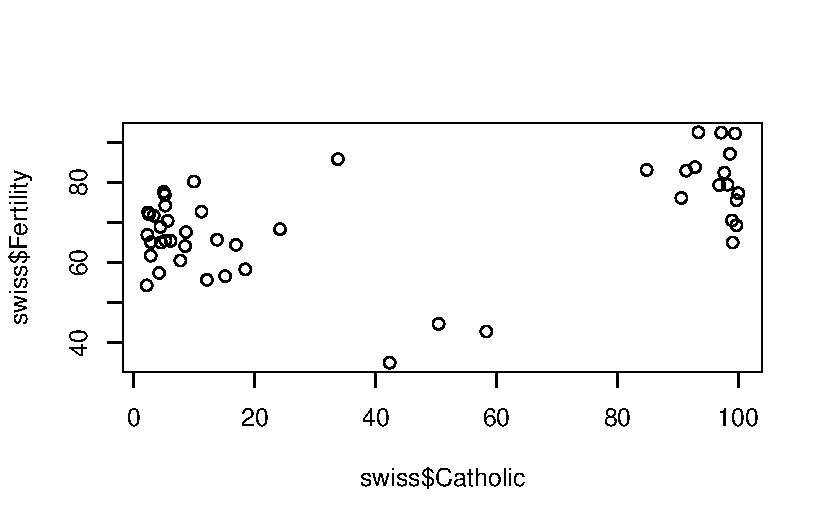
\includegraphics{paper_files/figure-pdf/fig-1-1.pdf}

}

\caption{\label{fig-1}Scatterplot of Speed and Distance}

\end{figure}

But it turns out that it doesn't always work so well.

\hypertarget{ggplot2-graphs}{%
\subsection{ggplot2 graphs}\label{ggplot2-graphs}}

Same is true for ggplot2 as you can see in Figure @ref(fig:fig-2).

\begin{figure}[H]

{\centering 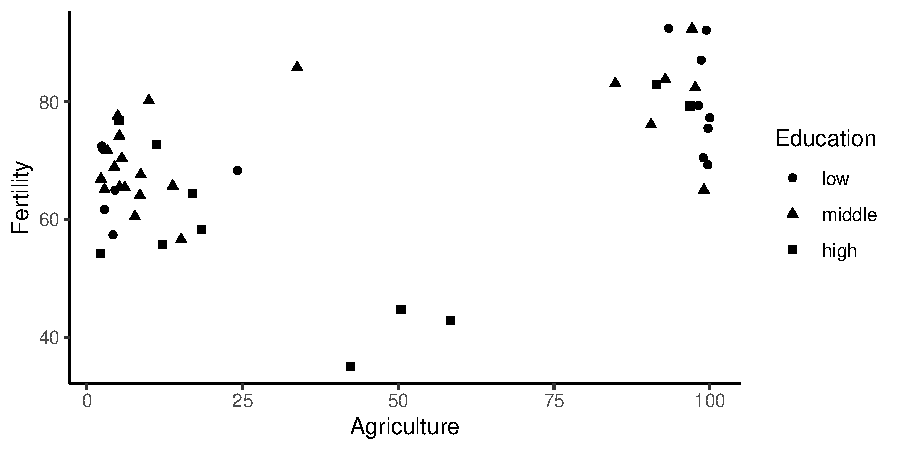
\includegraphics{paper_files/figure-pdf/fig-2-1.pdf}

}

\caption{\label{fig-2}Miles per gallon according to the weight}

\end{figure}

\hypertarget{compiling-the-document}{%
\section{Compiling the document}\label{compiling-the-document}}

To view your paper, pagedown requires a web server (since it is based on
paged.js)\footnote{open-source library to paginate content in the
  browser}. By compiling a document, R Studio will display your HTML
page through a local web server, i.e., paged.js will work in RStudio
Viewer.

There are several options, depending on your intention:

\begin{itemize}
\item
  click on the \texttt{Knit} button in R Studio which by default will
  provide a HTML document in the RStudio viewer pane (the HTML will be
  stored in your working directory)
\item
  use pagedown's \texttt{chrome\_print} function in the YAML (uncomment
  line \#24 of this \texttt{Rmd} file) if additionally you want your
  HTML based web page to be printed to be PDF (the PDF will be stored in
  your working directory)
\item
  to ``live''-preview your pages do not click on the \texttt{Knit}
  button but use the \textbf{xaringan} (Xie 2021) RStudio add-in
  \emph{Infinite Moon Reader}. You can simply call the function
  \texttt{xaringan::inf\_mr()} (within your console). This will launch a
  local web server via the \textbf{servr} package (Xie 2021a) and
  display your pages in the RStudio viewer. Each time you save your
  document (\emph{Ctrl+S}) xaringan updates your pages in the viewer.
\item
  If you use the option \texttt{self\_contained:\ false} (see line \#21
  of this \texttt{Rmd} file) (change to true for a self-contained
  document, but it'll be a litte slower for Pandoc to render), don't
  click on the \texttt{Knit} button in RStudio. Use instead the
  \textbf{xaringan} (Xie 2021) RStudio add-in \emph{Infinite Moon
  Reader}.
\end{itemize}

\hypertarget{good-practices-for-reproducibility}{%
\section{Good practices for
reproducibility}\label{good-practices-for-reproducibility}}

Every researcher has his own optimized setup. Currently we would
recommend the following:

\begin{itemize}
\tightlist
\item
  Keep all files of your project (that matter for producing the PDF) in
  one folder without subfolders. You can zip and directly upload that
  folder to the \href{https://dataverse.harvard.edu/}{Harvard
  dataverse}.\footnote{Another good folder setup would be to store all
    files needed as input files for the R Markdown manuscript in a
    subfolder called ``input'' and all output files that are produced
    apart from paper.html and paper.pdf in a subfolder called
    ``output''.}
\item
  Make sure that filenames have a logic to them.

  \begin{itemize}
  \tightlist
  \item
    Main file with text/code: ``paper.rmd'', ``report.rmd''
  \item
    Data files: ``data\_xxxxxx.*''
  \item
    Image files: ``fig\_xxxxxx.*''
  \item
    Tables files: ``table\_xxxx.*''
  \item
    etc.
  \item
    Ideally, your filenames will correspond to the names in the paper.
    For instance, Figure 1 in the paper may have a corresponding file
    called \texttt{fig\_1\_xxxxx.pdf}.
  \end{itemize}
\item
  Use the document outline in R studio (Ctrl + Shift + O) when you work
  with R Markdown.
\item
  Name rchunks according to what they do or produce:

  \begin{itemize}
  \tightlist
  \item
    ``\texttt{fig-...}'' for chunks producing figures
  \item
    ``\texttt{table-...}'' for chunks producing tables
  \item
    ``\texttt{model-...}'' for chunks producing model estimates
  \item
    ``\texttt{import-...}'' for chunks importing data
  \item
    ``\texttt{recoding-...}'' for chunks in which data is recoded
  \end{itemize}
\item
  Use ``really'' informative variable names:

  \begin{itemize}
  \tightlist
  \item
    Q: What do you think does the variable \emph{trstep} measure? It
    actually measures trust in the European parliament.

    \begin{itemize}
    \tightlist
    \item
      How could we call this variable instead? Yes,
      \texttt{trust.european.parliament} which is longer but will
      probably be understood by another researcher in 50 years.
    \end{itemize}
  \item
    If your setup is truly reproducible you will probably re-use the
    variable names that you generate as variable names in the tables you
    produce. Hence, there is an incentive to use good names.
  \end{itemize}
\item
  Use unique identifiers in the final R Markdown document paper.rmd that
  you upload:

  \begin{itemize}
  \tightlist
  \item
    Think of someone who wants to produce Figure 1/Model 1/Table 1 in
    your paper but doesn't find it in your code\ldots{}

    \begin{itemize}
    \tightlist
    \item
      Name the chunks ``fig-1'', ``fig-2'' as the are named in the
      published paper.
    \item
      Name the chunks that produce tables ``table-1'', ``table-2'' etc.
      as they are named in the published paper.
    \item
      Name your statistical models in your R code ``M1'', ``M2'' as they
      are named in the published paper.
    \end{itemize}
  \end{itemize}
\end{itemize}

\hypertarget{additional-tricks-for-publishing}{%
\section{Additional tricks for
publishing}\label{additional-tricks-for-publishing}}

\begin{itemize}
\tightlist
\item
  Make your script anonymous

  \begin{itemize}
  \tightlist
  \item
    Simply put a \texttt{\textless{}!-\/-\ ...\ -\/-\textgreater{}}
    around any identifying information, e.g., author names, title
    footnote etc.
  \end{itemize}
\item
  Counting words

  \begin{itemize}
  \tightlist
  \item
    Use adobe acrobat (commerical software) to convert your file to a
    word file. Then open in word and delete all the parts that shouldn't
    go into the word count. The word count is displayed in the lower
    right.
  \item
    Use an one of the online services to count your words (search for
    ``pdf word count'')
  \end{itemize}
\item
  Appendix: You can change the numbering format for the appendix in the
  rmd file

  \begin{itemize}
  \tightlist
  \item
    What is still not possible in this document is to automatically have
    separate reference sections for paper and appendix.
  \end{itemize}
\item
  Journals may require you to use their tex style: Sometimes you can
  simply use their template in your rmarkdown file. See
  \href{https://dataverse.harvard.edu/dataset.xhtml?persistentId=doi:10.7910/DVN/LDUMNY}{here}
  for a PLOS one example.
\end{itemize}

\hypertarget{citation-styles}{%
\section{Citation styles}\label{citation-styles}}

If your study needs to follow a particular citation style, you can set
the corresponding style in the header of your \texttt{.rmd} document. To
do so you have to download the corresponding \texttt{.csl} file.

In the present document we use the style of the American Sociological
Association and set it in the preamble with
\texttt{csl:\ american-sociological-association.csl}. However, you also
need to download the respective \texttt{.csl} file from the following
github page: https://github.com/citation-style-language/styles and copy
it into your working directory for it to work.

The github directory contains a wide variety of citation style files
depending on what discipline you work in.

\newpage

\hypertarget{references}{%
\section*{References}\label{references}}
\addcontentsline{toc}{section}{References}

\hypertarget{refs}{}
\begin{CSLReferences}{1}{0}
\leavevmode\vadjust pre{\hypertarget{ref-Bauer2018-dl}{}}%
Bauer, Paul. 2018. {``Writing a Reproducible Paper in {R} Markdown.''}
\emph{Open Science Framework Preprint}, December, 1--14.

\leavevmode\vadjust pre{\hypertarget{ref-Kirsop2005-ro}{}}%
Kirsop, Barbara, and Leslie Chan. 2005. {``Transforming Access to
Research Literature for Developing Countries.''} \emph{Serials Review}
31 (4): 246--55.

\leavevmode\vadjust pre{\hypertarget{ref-R2017}{}}%
R Core Team. 2017. \emph{R: A Language and Environment for Statistical
Computing}. Vienna, Austria: R Foundation for Statistical Computing.
\url{https://www.R-project.org/}.

\leavevmode\vadjust pre{\hypertarget{ref-Rstudio2015}{}}%
RStudio Team. 2015. \emph{RStudio: Integrated Development Environment
for r}. Boston, MA: RStudio, Inc. \url{http://www.rstudio.com/}.

\leavevmode\vadjust pre{\hypertarget{ref-knitr3}{}}%
Xie, Yihui. 2014. {``Knitr: A Comprehensive Tool for Reproducible
Research in {R}.''} In \emph{Implementing Reproducible Computational
Research}, edited by Victoria Stodden, Friedrich Leisch, and Roger D.
Peng. Chapman; Hall/CRC.
\url{http://www.crcpress.com/product/isbn/9781466561595}.

\leavevmode\vadjust pre{\hypertarget{ref-knitr2}{}}%
---------. 2015. \emph{Dynamic Documents with {R} and Knitr}. 2nd ed.
Boca Raton, Florida: Chapman; Hall/CRC. \url{https://yihui.name/knitr/}.

\leavevmode\vadjust pre{\hypertarget{ref-bookdown2}{}}%
---------. 2016. \emph{Bookdown: Authoring Books and Technical Documents
with {R} Markdown}. Boca Raton, Florida: Chapman; Hall/CRC.
\url{https://github.com/rstudio/bookdown}.

\leavevmode\vadjust pre{\hypertarget{ref-bookdown1}{}}%
---------. 2017. \emph{Bookdown: Authoring Books and Technical Documents
with r Markdown}. \url{https://github.com/rstudio/bookdown}.

\leavevmode\vadjust pre{\hypertarget{ref-knitr1}{}}%
---------. 2018. \emph{Knitr: A General-Purpose Package for Dynamic
Report Generation in r}. \url{https://yihui.name/knitr/}.

\leavevmode\vadjust pre{\hypertarget{ref-xaringan}{}}%
---------. 2021. \emph{Xaringan: Presentation Ninja}.
\url{https://CRAN.R-project.org/package=xaringan}.

\leavevmode\vadjust pre{\hypertarget{ref-Xie2021-bi}{}}%
Xie, Yihui, and Romain Lesur. 2021. {``Pagedown: Create Paged {HTML}
Documents for Printing from {R} Markdown.''}
\url{https://rstudio.github.io/pagedown/}.

\leavevmode\vadjust pre{\hypertarget{ref-Xie2021-ls}{}}%
Xie, Yihui, Romain Lesur, Brent Thorne, and Xianying Tan. 2021.
\emph{Pagedown: Paginate the HTML Output of r Markdown with CSS for
Print}. \url{https://CRAN.R-project.org/package=pagedown}.

\leavevmode\vadjust pre{\hypertarget{ref-kableextra}{}}%
Zhu, Hao. 2017. \emph{kableExtra: Construct Complex Table with 'Kable'
and Pipe Syntax}. \url{https://CRAN.R-project.org/package=kableExtra}.

\end{CSLReferences}

\newpage

\hypertarget{online-appendix}{%
\section*{Online appendix}\label{online-appendix}}
\addcontentsline{toc}{section}{Online appendix}

\hypertarget{sec:rsessioninfo}{%
\subsection{Attach R session info in appendix}\label{sec:rsessioninfo}}

Since R and R packages are constantly evolving you might want to add the
R session info that contains information on the R version as well as the
packages that are loaded.

\begin{verbatim}
R version 4.2.2 (2022-10-31 ucrt)
Platform: x86_64-w64-mingw32/x64 (64-bit)
Running under: Windows 10 x64 (build 17763)

Matrix products: default

attached base packages:
[1] stats     graphics  grDevices utils     datasets  methods   base     

other attached packages:
[1] ggplot2_3.4.1      gt_0.8.0           dplyr_1.1.0        gdtools_0.3.0     
[5] flextable_0.8.5    modelsummary_1.3.0 kableExtra_1.3.4   knitr_1.42        

loaded via a namespace (and not attached):
 [1] Rcpp_1.0.10        svglite_2.1.1      digest_0.6.31      utf8_1.2.3        
 [5] mime_0.12          R6_2.5.1           backports_1.4.1    evaluate_0.20     
 [9] httr_1.4.4         highr_0.10         pillar_1.8.1       rlang_1.0.6       
[13] curl_5.0.0         uuid_1.1-0         performance_0.10.2 rstudioapi_0.14   
[17] data.table_1.14.6  checkmate_2.1.0    rmarkdown_2.20     labeling_0.4.2    
[21] webshot_0.5.4      stringr_1.5.0      munsell_0.5.0      shiny_1.7.4       
[25] compiler_4.2.2     httpuv_1.6.9       xfun_0.37          parameters_0.20.2 
[29] pkgconfig_2.0.3    askpass_1.1        systemfonts_1.0.4  base64enc_0.1-3   
[33] gfonts_0.2.0       htmltools_0.5.4    insight_0.19.0     openssl_2.0.5     
[37] tidyselect_1.2.0   tibble_3.1.8       httpcode_0.3.0     fansi_1.0.4       
[41] viridisLite_0.4.1  withr_2.5.0        crayon_1.5.2       later_1.3.0       
[45] tables_0.9.10      crul_1.3           grid_4.2.2         gtable_0.3.1      
[49] jsonlite_1.8.4     xtable_1.8-4       lifecycle_1.0.3    bayestestR_0.13.0 
[53] magrittr_2.0.3     scales_1.2.1       datawizard_0.6.5   zip_2.2.2         
[57] cli_3.6.0          stringi_1.7.12     cachem_1.0.6       farver_2.1.1      
[61] promises_1.2.0.1   xml2_1.3.3         ellipsis_0.3.2     generics_0.1.3    
[65] vctrs_0.5.2        tools_4.2.2        glue_1.6.2         officer_0.5.2     
[69] fastmap_1.1.0      yaml_2.3.7         colorspace_2.1-0   rvest_1.0.3       
[73] memoise_2.0.1     
\end{verbatim}

\hypertarget{all-the-code-in-the-paper}{%
\subsection{All the code in the paper}\label{all-the-code-in-the-paper}}

To simply attach all the code you used in the PDF file in the appendix
see the R chunk in the underlying \texttt{.rmd} file:

\begin{Shaded}
\begin{Highlighting}[]
\NormalTok{knitr}\SpecialCharTok{::}\NormalTok{opts\_chunk}\SpecialCharTok{$}\FunctionTok{set}\NormalTok{(}\AttributeTok{cache =} \ConstantTok{FALSE}\NormalTok{)}
\CommentTok{\# Use chache = TRUE if you want to speed up compilation}
\CommentTok{\# A function to allow for showing some of the inline code}
\NormalTok{rinline }\OtherTok{\textless{}{-}} \ControlFlowTok{function}\NormalTok{(code)\{}
\NormalTok{  html }\OtherTok{\textless{}{-}} \StringTok{\textquotesingle{}\textless{}code  class="r"\textgreater{}\textasciigrave{}\textasciigrave{}\textasciigrave{} \textasciigrave{}r CODE\textasciigrave{} \textasciigrave{}\textasciigrave{}\textasciigrave{}\textless{}/code\textgreater{}\textquotesingle{}}
  \FunctionTok{sub}\NormalTok{(}\StringTok{"CODE"}\NormalTok{, code, html)}
\NormalTok{\}}
\NormalTok{remotes}\SpecialCharTok{::}\FunctionTok{install\_github}\NormalTok{(}\StringTok{\textquotesingle{}rstudio/pagedown\textquotesingle{}}\NormalTok{)}
\FunctionTok{install.packages}\NormalTok{(}\FunctionTok{c}\NormalTok{(}\StringTok{"rmarkdown"}\NormalTok{, }\StringTok{"knitr"}\NormalTok{, }\StringTok{"kableExtra"}\NormalTok{,}
                   \StringTok{"stargazer"}\NormalTok{, }\StringTok{"modelsummary"}\NormalTok{, }\StringTok{"knitr"}\NormalTok{, }\StringTok{"gt"}\NormalTok{))}
\FunctionTok{cat}\NormalTok{(}\FunctionTok{paste}\NormalTok{(}\StringTok{"\#"}\NormalTok{, }\FunctionTok{capture.output}\NormalTok{(}\FunctionTok{sessionInfo}\NormalTok{()), }\StringTok{"}\SpecialCharTok{\textbackslash{}n}\StringTok{"}\NormalTok{, }\AttributeTok{collapse =}\StringTok{""}\NormalTok{)) }
  \CommentTok{\# or use message() instead of cat()}
\NormalTok{x }\OtherTok{\textless{}{-}} \DecValTok{1}\SpecialCharTok{:}\DecValTok{10}
\NormalTok{x}
\NormalTok{data }\OtherTok{\textless{}{-}} \FunctionTok{read.csv}\NormalTok{(}\StringTok{"data.csv"}\NormalTok{)}
\FunctionTok{head}\NormalTok{(data)}
\FunctionTok{dput}\NormalTok{(data[}\DecValTok{1}\SpecialCharTok{:}\DecValTok{5}\NormalTok{,]) }\CommentTok{\# here we only take a subset}
\NormalTok{data }\OtherTok{\textless{}{-}} \FunctionTok{structure}\NormalTok{(}\FunctionTok{list}\NormalTok{(}\AttributeTok{Fertility =} \FunctionTok{c}\NormalTok{(}\FloatTok{80.2}\NormalTok{, }\FloatTok{83.1}\NormalTok{, }\FloatTok{92.5}\NormalTok{, }\FloatTok{85.8}\NormalTok{, }\FloatTok{76.9}\NormalTok{), }\AttributeTok{Agriculture =} \FunctionTok{c}\NormalTok{(}\DecValTok{17}\NormalTok{, }
\FloatTok{45.1}\NormalTok{, }\FloatTok{39.7}\NormalTok{, }\FloatTok{36.5}\NormalTok{, }\FloatTok{43.5}\NormalTok{), }\AttributeTok{Examination =} \FunctionTok{c}\NormalTok{(15L, 6L, 5L, 12L, 17L}
\NormalTok{), }\AttributeTok{Education =} \FunctionTok{c}\NormalTok{(12L, 9L, 5L, 7L, 15L), }\AttributeTok{Catholic =} \FunctionTok{c}\NormalTok{(}\FloatTok{9.96}\NormalTok{, }\FloatTok{84.84}\NormalTok{, }
\FloatTok{93.4}\NormalTok{, }\FloatTok{33.77}\NormalTok{, }\FloatTok{5.16}\NormalTok{), }\AttributeTok{Infant.Mortality =} \FunctionTok{c}\NormalTok{(}\FloatTok{22.2}\NormalTok{, }\FloatTok{22.2}\NormalTok{, }\FloatTok{20.2}\NormalTok{, }\FloatTok{20.3}\NormalTok{, }
\FloatTok{20.6}\NormalTok{)), }\AttributeTok{class =} \StringTok{"data.frame"}\NormalTok{, }\AttributeTok{row.names =} \FunctionTok{c}\NormalTok{(}\ConstantTok{NA}\NormalTok{, }\SpecialCharTok{{-}}\NormalTok{5L))}
\FunctionTok{library}\NormalTok{(knitr)}
\FunctionTok{library}\NormalTok{(kableExtra)}

\FunctionTok{kable}\NormalTok{(swiss[}\DecValTok{1}\SpecialCharTok{:}\DecValTok{10}\NormalTok{,], }\AttributeTok{row.names =} \ConstantTok{TRUE}\NormalTok{, }
      \AttributeTok{caption =} \StringTok{\textquotesingle{}Table with kable() and kablestyling()\textquotesingle{}}\NormalTok{, }
      \AttributeTok{format =} \StringTok{"html"}\NormalTok{, }\AttributeTok{booktabs =}\NormalTok{ T) }\SpecialCharTok{\%\textgreater{}\%}
        \FunctionTok{kable\_styling}\NormalTok{(}\AttributeTok{full\_width =}\NormalTok{ T, }
                      \AttributeTok{latex\_options =} \FunctionTok{c}\NormalTok{(}\StringTok{"striped"}\NormalTok{, }
                                        \StringTok{"scale\_down"}\NormalTok{,}
                                        \StringTok{"HOLD\_position"}\NormalTok{),}
                      \AttributeTok{font\_size =} \DecValTok{10}\NormalTok{)}


\FunctionTok{library}\NormalTok{(modelsummary)}
\FunctionTok{datasummary\_skim}\NormalTok{(swiss, }
                 \AttributeTok{type=}\StringTok{"numeric"}\NormalTok{, }
                 \AttributeTok{histogram=}\NormalTok{T, }
                 \AttributeTok{title =} \StringTok{"Summary: Numeric variables"}\NormalTok{)}
\CommentTok{\# Create categorical variables}
\NormalTok{swiss}\SpecialCharTok{$}\NormalTok{Education\_cat }\OtherTok{\textless{}{-}} \FunctionTok{cut}\NormalTok{(swiss}\SpecialCharTok{$}\NormalTok{Education, }
                   \AttributeTok{breaks=}\FunctionTok{c}\NormalTok{(}\SpecialCharTok{{-}}\ConstantTok{Inf}\NormalTok{, }\DecValTok{6}\NormalTok{, }\DecValTok{12}\NormalTok{, }\ConstantTok{Inf}\NormalTok{), }
                   \AttributeTok{labels=}\FunctionTok{c}\NormalTok{(}\StringTok{"low"}\NormalTok{,}\StringTok{"middle"}\NormalTok{,}\StringTok{"high"}\NormalTok{))}
\NormalTok{swiss}\SpecialCharTok{$}\NormalTok{Infant.Mortality\_cat }\OtherTok{\textless{}{-}} \FunctionTok{cut}\NormalTok{(swiss}\SpecialCharTok{$}\NormalTok{Infant.Mortality, }
                   \AttributeTok{breaks=}\FunctionTok{c}\NormalTok{(}\SpecialCharTok{{-}}\ConstantTok{Inf}\NormalTok{, }\FloatTok{18.15}\NormalTok{, }\FloatTok{21.70}\NormalTok{, }\ConstantTok{Inf}\NormalTok{), }
                   \AttributeTok{labels=}\FunctionTok{c}\NormalTok{(}\StringTok{"low"}\NormalTok{,}\StringTok{"middle"}\NormalTok{,}\StringTok{"high"}\NormalTok{))}

\FunctionTok{library}\NormalTok{(flextable)}
\NormalTok{tab\_cat }\OtherTok{\textless{}{-}} \FunctionTok{datasummary\_skim}\NormalTok{(swiss, }
                            \AttributeTok{type=}\StringTok{"categorical"}\NormalTok{, }
                            \AttributeTok{title =} \StringTok{"Summary: Categorical variables"}\NormalTok{,}
                            \AttributeTok{output =} \StringTok{\textquotesingle{}flextable\textquotesingle{}}\NormalTok{)}

\CommentTok{\# additionally we want to change the font, fontsize and spacing}
\FunctionTok{library}\NormalTok{(}\StringTok{"gdtools"}\NormalTok{)}

\FunctionTok{library}\NormalTok{(dplyr)}
\NormalTok{tab\_cat }\OtherTok{\textless{}{-}}\NormalTok{ tab\_cat }\SpecialCharTok{\%\textgreater{}\%}
  \FunctionTok{font}\NormalTok{(}\AttributeTok{fontname=}\StringTok{"Times New Roman"}\NormalTok{, }\AttributeTok{part=}\StringTok{"header"}\NormalTok{) }\SpecialCharTok{\%\textgreater{}\%}
  \FunctionTok{font}\NormalTok{(}\AttributeTok{fontname=}\StringTok{"Times New Roman"}\NormalTok{, }\AttributeTok{j=}\DecValTok{1}\SpecialCharTok{:}\DecValTok{4}\NormalTok{) }\SpecialCharTok{\%\textgreater{}\%} 
  \FunctionTok{fontsize}\NormalTok{(}\AttributeTok{size=}\DecValTok{12}\NormalTok{, }\AttributeTok{part=}\StringTok{"header"}\NormalTok{) }\SpecialCharTok{\%\textgreater{}\%}
  \FunctionTok{fontsize}\NormalTok{(}\AttributeTok{size=}\DecValTok{10}\NormalTok{, }\AttributeTok{j=}\DecValTok{1}\SpecialCharTok{:}\DecValTok{4}\NormalTok{) }\SpecialCharTok{\%\textgreater{}\%} 
  \FunctionTok{line\_spacing}\NormalTok{(}\AttributeTok{space =} \FloatTok{0.3}\NormalTok{, }\AttributeTok{part =} \StringTok{"all"}\NormalTok{)}

\NormalTok{tab\_cat}
\FunctionTok{library}\NormalTok{(modelsummary)}
\NormalTok{M1 }\OtherTok{\textless{}{-}} \FunctionTok{lm}\NormalTok{(Fertility }\SpecialCharTok{\textasciitilde{}}\NormalTok{ Education }\SpecialCharTok{+}\NormalTok{ Agriculture, }\AttributeTok{data =}\NormalTok{ swiss)}
\NormalTok{M2 }\OtherTok{\textless{}{-}} \FunctionTok{lm}\NormalTok{(Fertility }\SpecialCharTok{\textasciitilde{}}\NormalTok{ Education }\SpecialCharTok{+}\NormalTok{ Catholic, }\AttributeTok{data =}\NormalTok{ swiss)}
\NormalTok{M3 }\OtherTok{\textless{}{-}} \FunctionTok{lm}\NormalTok{(Fertility }\SpecialCharTok{\textasciitilde{}}\NormalTok{ Education }\SpecialCharTok{+}\NormalTok{ Infant.Mortality }\SpecialCharTok{+}\NormalTok{ Agriculture, }\AttributeTok{data =}\NormalTok{ swiss)}
\NormalTok{models }\OtherTok{\textless{}{-}} \FunctionTok{list}\NormalTok{(}\StringTok{"M1"} \OtherTok{=}\NormalTok{ M1, }\StringTok{"M2"} \OtherTok{=}\NormalTok{  M2, }\StringTok{"M3"} \OtherTok{=}\NormalTok{ M3)}


\FunctionTok{library}\NormalTok{(gt)}
\CommentTok{\# additionally we want to change the font, font size and spacing}
\FunctionTok{modelsummary}\NormalTok{(models,}
             \AttributeTok{title =} \StringTok{\textquotesingle{}Linear regression\textquotesingle{}}\NormalTok{,}
             \AttributeTok{output =} \StringTok{\textquotesingle{}gt\textquotesingle{}}\NormalTok{,}
             \AttributeTok{notes =} \StringTok{"Notes: some notes..."}\NormalTok{) }\SpecialCharTok{\%\textgreater{}\%}
    \FunctionTok{tab\_spanner}\NormalTok{(}\AttributeTok{label =} \StringTok{\textquotesingle{}Dependent variable: Fertility\textquotesingle{}}\NormalTok{, }\AttributeTok{columns =} \DecValTok{2}\SpecialCharTok{:}\DecValTok{4}\NormalTok{) }\SpecialCharTok{\%\textgreater{}\%}
  \FunctionTok{tab\_options}\NormalTok{(}
    \AttributeTok{table.font.size =} \DecValTok{10}\NormalTok{,}
    \AttributeTok{data\_row.padding =} \FunctionTok{px}\NormalTok{(}\DecValTok{1}\NormalTok{),}
    \AttributeTok{table.border.top.color =} \StringTok{"white"}\NormalTok{,}
    \AttributeTok{heading.border.bottom.color =} \StringTok{"black"}\NormalTok{,}
    \AttributeTok{row\_group.border.top.color =} \StringTok{"black"}\NormalTok{,}
    \AttributeTok{row\_group.border.bottom.color =} \StringTok{"white"}\NormalTok{,}
    \AttributeTok{table.border.bottom.color =} \StringTok{"white"}\NormalTok{,}
    \AttributeTok{column\_labels.border.top.color =} \StringTok{"black"}\NormalTok{,}
    \AttributeTok{column\_labels.border.bottom.color =} \StringTok{"black"}\NormalTok{,}
    \AttributeTok{table\_body.border.bottom.color =} \StringTok{"black"}\NormalTok{,}
    \AttributeTok{table\_body.hlines.color =} \StringTok{"white"}
\NormalTok{  )}


\FunctionTok{plot}\NormalTok{(swiss}\SpecialCharTok{$}\NormalTok{Catholic, swiss}\SpecialCharTok{$}\NormalTok{Fertility)}
\FunctionTok{library}\NormalTok{(ggplot2)}
\FunctionTok{ggplot}\NormalTok{(swiss, }\FunctionTok{aes}\NormalTok{(}\AttributeTok{x=}\NormalTok{Catholic, }\AttributeTok{y=}\NormalTok{Fertility, }\AttributeTok{shape=}\NormalTok{Education\_cat)) }\SpecialCharTok{+} \FunctionTok{geom\_point}\NormalTok{() }\SpecialCharTok{+}
  \FunctionTok{labs}\NormalTok{(}\AttributeTok{x=}\StringTok{"Agriculture"}\NormalTok{, }\AttributeTok{y =} \StringTok{"Fertility"}\NormalTok{, }
       \AttributeTok{shape=}\StringTok{"Education"}\NormalTok{) }\SpecialCharTok{+} \FunctionTok{theme\_classic}\NormalTok{()}
\FunctionTok{print}\NormalTok{(}\FunctionTok{sessionInfo}\NormalTok{(), }\AttributeTok{local =} \ConstantTok{FALSE}\NormalTok{)}
\end{Highlighting}
\end{Shaded}




\end{document}
